% !TEX root = ../thesis.tex

\chapter{Polyhedra Analysis}
\mbox{}\\
\mbox{}\\
\mbox{}\\
Polyhedra analysis is one of the main tools of static analysis \cite{cousot1977abstract}. During the execution of a program, its statements and expressions can create relationships between the different variables of the program. Polyhedra are the most expressive way of modelling all these different relations. Even though alternatives for constraint representation exist, none are as expressive as polyhedra. Unfortunately, this domain has worst-case exponential space and time complexity, meaning that using it on most real-world sized applications would very often cause it to either timeout or run out of memory making it very impractical. Therefore, other domains have been more widely used, such as Octagon \cite{mine2006octagon}, Zone \cite{mine2001new} or Pentagon \cite{logozzo2010pentagons}, but all of these are less expressive and therefore less precise by design. In recent years, several techniques have been developed that have managed to speed up polyhedra analysis without causing it to lose precision \cite{gange2016exploiting,jourdan2017sparsity,marechal2017efficient}. Some of these methods are implemented inside the ELINA framework. We shall now briefly present the methods that are relevant to this work.
\section{Polyhedra representation}
One of the techniques used to increase the performance of static analysis involves the way in which we represent our domain \cite{singh2015making}. Polyhedra, for example, can be represented with both the constraint representation and the generator representation \cite{motzkin1953double}. To illustrate these different representations I will proceed with the following example. Let's assume we have the following statement:
\paragraph{Example 3.1}\mbox{}\\
\begin{center}
	$if \; x\geq1\wedge y \geq 1 \wedge x - y \leq 0: $\\ 
	$...\;\;\;\;\;$\\
	$end \qquad\qquad\qquad\qquad\qquad\qquad$
\end{center}

Inside of the if statement, the polyhedron would have the following shape:

\begin{figure}[h]
\begin{center}
	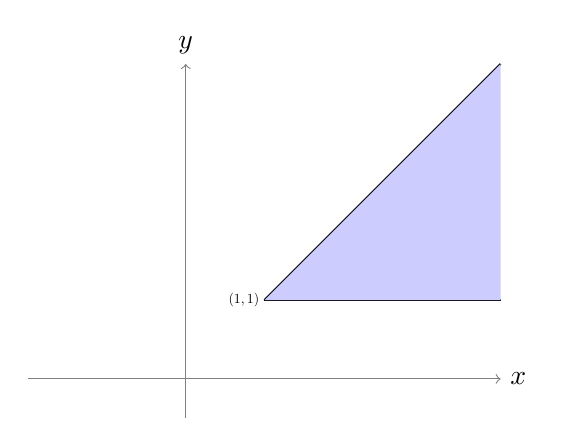
\begin{tikzpicture}
    \draw [thin, gray, ->] (0,-0.5) -- (0,4)      % draw y-axis line
        node [above, black] {$y$};              % add label for y-axis

    \draw [thin, gray, ->] (-2,0) -- (4,0)      % draw x-axis line
        node [right, black] {$x$};             % add label for x-axis

    \draw [draw=black,thick] (4.,4.) -- (1,1)% draw the graph
   	 	node [left, black, scale =0.5] {$(1,1)$};
    \draw [draw=black,thick] (1,1) -- (4.,1) 
    	node [right, black, scale =0.5] {};
    \fill[fill=blue!20] (1,1)--(4.,4.)--(4.,1);  
	\end{tikzpicture}
	\caption{Example of a polyhedron modelling the above constraints}

\end{center}
\end{figure}
\mbox{}\\

There are two ways for us to represent this information.
\subsection{Constraint representation}
In constraint representation, we model the polyhedron as the intersection of a finite number of closed half spaces and a finite number of subspaces. The resulting polyhedron can be written as:

\begin{equation}
    P=\{x\in Q^n |Ax\leq b \wedge Dx=e\}
\end{equation}
where A,D are matrices and b,e are vectors of natural numbers. Therefore, the constraint representation of the above example would be:

\begin{equation}
    C = \{-x \leq -1, -y \leq -1, x\leq y \} 
\end{equation}

\subsection{Generator representation}
In order to encode a Polyhedron with the generator representation, we have to model it as the convex hull of three items: 

%TODO finish list with rep 
\begin{itemize}
    \item A finite set $V\in Q^n$ of vertices $v_i \in V$.
    \item A finite set $R \subseteq Q^n$ of rays. $r_i \in R$ are direction vectors of infinite edges of the polyhedron with one end bounded. Each ray starts from a $v \in V$.
    \item  A finite set $Z \subseteq Q^n$ of lines. $z_i \in Z$ are direction vectors of infinite edges of the polyhedron with both ends unbounded. Each line passes through a $v \in V$.
\end{itemize}Inside of the if statement, the polyhedron would have the following shape:
%TODO finish example
The result of generator representation on the previous example would have the following form: 
\begin{equation}
    G = \{ V = \{(1,1)\}, R = \{(1,1),(1,0) \}, Z = \emptyset \}
\end{equation}
\subsection{Polyhedra domain}
Once we can represent our polyhedra, to make them useful, a set of operators has to be defined as well. The polyhedra abstract domain consists of the polyhedral lattice:
    $(P,\sqsubseteq,\sqcup,\sqcap,\perp,\top)$, and a set of operators that we can apply on them. The different operators are the following:
    \begin{itemize}
        \item Inclusion test: $P \sqsubseteq Q$, holds if all generators in $G_P$ satisfy all constraint in $C_Q$
        \item Equality test: $P=Q$, checks whether the polyhedra are equal
        \item Join: $P\sqcup Q$, $G_{output}$ is the union of the generators from the input. $C_{output}$ is obtained by incrementally adding the generators from $G_Q$ to the polyhedron defined by $C_P$
        \item Meet: $P\sqcap Q$, $C_{output}$ is the union of the constraints in the input polyhedra. $G_{output}$ is obtained by incrementally adding the constraints in $C_Q$ to the polyhedron defined by $G_P$
        \item Widening, this operator is applied to accelerate convergence since the polyhedral lattice has infinite height:
		\begin{center}
		  \[
    C_{P\nabla Q}=\left\{
                \begin{array}{ll}
                  C_Q $ if $P=\perp ;\\
                  C'_P\bigcup C'_Q, $ otherwise$;
                \end{array}
              \right.
  	\]
		
        \end{center}

        where $C'_p=\{c\in C_P |C_Q \vdash c \}$, and\\  $C'_Q=\{c\in C_Q |\exists c' \in C_P,C_P \vdash c $ and $((C_P\c')\bigcup \{c\})\vdash c' \}$
        where $C\vdash c$, tests wether c can be entailed from constraints in C
        \item Conditional: let $\otimes \in \{\leq,=\},1\leq 1\leq n,\alpha \in Q$ then $\alpha x_i \otimes \delta$ adds the constraint $(\alpha-a_i)x_i \otimes\delta - a_i x_i$ to the constraint set C
        \item Assignment: $x_i = \delta$, first adds $x_i$ to P then augments C with $x_i -\delta = 0$
        
    \end{itemize}
     In the following table, we can see the respective complexities of the different operators according to the representation
	 
\begin{center}
\begin{tabular}{||c c c c||} 
 
 \hline
 Operator & Constraint & Generator & Both \\ [0.5ex] 
 \hline
 Inclusion $(\sqsubseteq)$ & $O(mLP(m,n))$ & $O(gLP(g,n))$ & $O(ngm)$ \\ 
 \hline
 Join $(\bigsqcup)$ & $O(nm^{2^{n+1}})$ & $O(ng)$ & $O(ng)$ \\
 \hline
 Meet $(\sqcap)$ & $O(nm)$ & $O(ng^{2^{n+1}})$ & $O(nm)$\\
 \hline
 Widening $(\bigtriangledown)$ & $O(mLP(m,n))$ & $O(gLP(g,n))$ & $O(ngm)$ \\
 \hline
 Conditional & $O(n)$ & $O(ng^{2^{n+1}})$ & $O(n)$ \\ 
 \hline
 Assignment & $O(nm^2)$ & $O(ng)$ & $O(ng)$ \\ 
 
 
 \hline
\end{tabular}
\end{center}
$m=|C|,g=|G|,LP(m,n)$ is the complexity of solving a linear program with m constraints and n variables\\
As we can see, no representation is less complex than the other, as some of the operators are faster in one but others in the other. But, as we can see in the last table, when both representations are available all the operators have a polynomial complexity.\\
\subsubsection{Chernikova's Algorithm}
 The first optimisation that one can do is to keep both representations of the polyhedron and for each operator pick the representation that minimises the time complexity. A conversion between the two representations is possible thanks to Chernikova's algorithm \cite{chernikova1968algorithm}. However, Chernikova's algorithm still has worst-case exponential complexity and it becomes the new bottleneck for the double representation.
 
 \section{Polyhedra Decomposition}
Another technique used for increasing the efficiency of polyhedra analysis is the use of online decomposition \cite{singh2017fast}. It is based on the observation that during the execution of a program, not all its variables are dependent on one another. Using this observation, we can separate the set of all variables into smaller, independent sets. Therefore, instead of representing the whole set of variables with one large polyhedron, we can instead represent it with various smaller ones.\\ Let's assume we have a set of variables $\chi$ in a Polyhedron $P$. The set $\chi$ can be partitioned as $\pi_P=\{ \chi_1,\chi_2,..,\chi_r\}$, $\chi_i\subseteq\chi $. We call the partitioning of the set permissible if no two variables $x_i$ and $x_j$ exist that are in different blocks in $\pi$ and are related by a constraint in P. We call the $\top$ partition, a partition where all the variables are in one block, i.e no partitioning is done. Similarly, the $\perp$ partition is a partition where each variable has its own block, i.e all variables are independent of one another. Once the decomposition has been done in this way, during the execution of an operator, it only has to be executed on the subset of blocks that contain the same variables. This allows for a very large performance gain in both space and time, giving us the following time complexity for the various operators.

\paragraph{Table 2} Asymptotic time complexity of Polyhedra domain operators with decomposition

\begin{center}
\begin{tabular}{||c c||} 
 
 \hline
 Operator & Decomposed  \\ [0.5ex] 
 \hline
 Inclusion $(\sqsubseteq)$ & $O(\sum_{i=1}^r n_ig_im_i)$\\ 
 \hline
 Join $(\bigsqcup)$ & $O(\sum_{i=1}^r n_i g_i m_i + n_{max} g_{max})$ \\
 \hline
 Meet $(\sqcap)$ & $O(\sum_{i=1}^r n_i m_i)$ \\
 \hline
 Widening $(\bigtriangledown)$ & $O(\sum_{i=1}^r n_i g_i m_i)$\\
 \hline
 Conditional & $O(n_{max})$ \\ 
 \hline
 Assignment & $O(n_{max}g_{max})$ \\ 
 
 
 \hline
\end{tabular}
\end{center}

 
\paragraph{Example 3.2} \mbox{}\\
Let's consider the variables $X = \{x_1,x_2,x_3,x_4\}$ and $C = \{ x_1 + 2 \cdot x_3 \leq 10, x_2 = 1 \}$.\\
This polyhedron can be partitioned into three blocks $\pi_P = \{\{x_1,x_3\},\{x_2\},\{x_4\}\}$ and the constraints of the corresponding blocks are equal to: 
\begin{center}
	$C_{P_1}\{x_1 + 2\cdot x_3 \leq 10 \} , C_{P_2}\{x_2 = 10 \}$
\end{center}

% TODO write example

\subsubsection{Operator decomposition}
As we change the model of our domain we must also update the operators inside this domain. For the sake of brevity, I will not go into detail about each of them, but I will concentrate on the join operator as it plays an important role in this paper.\\
During the execution of the join of $P$ and $Q$, the join operator can cause the creation of constraints between different blocks of $\pi_P$ and $\pi_Q$. In the worst case, all the blocks can be merged creating the $\top$ partition. In order to reconstruct the $\top$ partition from the blocks the following formula is used:
\begin{equation}
    P = P_1 \Join P_2 \Join ... \Join P_r = (C_{P_1} \cup C_{P_2} \cup ... \cup C_{P_1}, G_{P_1} \times G_{P_2} \times  ... \times   G_{P_r})
\end{equation}
Due to the cartesian product, building the $\top$ partition can blow up the number of generators and cause the join to be a serious bottleneck of online decomposition.

\subsection{Reinforcement Learning for polyhedra analysis}
Both of the techniques presented in chapters 3.2 and 3.3 achieve considerable performance gain without having to sacrifice any precision. Unfortunately, at some point compromises have to be made. Analysers that tune the precision and cost based on the program they are analysing are called parametric program analysers. Several such approaches already exist. \cite{oh2015learning,liang2011learning,heo2016learning}.
As explained in section 3.3.1., one bad constraint can significantly decrease the performance of the whole program. The trick is being able to identify this constraint at the correct time. One of the explored solutions to this problem that we shall explore is training a reinforcement learning algorithm  that will make the decisions of when and how to apply some abstractions \cite{singh2018fast}.\\
Intuitively, using reinforcement learning for polyhedra analysis seems quite straightforward. Let's imagine that for the join operator that we have presented above, we have two different versions $J_{pr}$ and $J_{pe}$. One of these is a slower and more precise join and the other, using some sort of abstraction, is faster but not as precise. The goal of the reinforcement learning method would then simply be to select the correct operator at the right time, thus enabling us to obtain the most precise result in a minimal time. Before this can be done, it is first necessary to initialise polyhedra analysis for reinforcement learning.

\subsubsection{Adapting polyhedra analysis for Reinforcement Learning}
As explained in section 2.1., reinforcement learning uses a defined set of concepts. In some way, these concepts have to be translated into the domain of polyhedra analysis. A possible mapping can be done in the following way.
\begin{center}
\begin{tabular}{||c c||} 
 \hline
 RL concept & Polyhedra analysis concept  \\ [0.5ex] 
 \hline
 \hline
 Agent & Static analyser\\ 

 State $s\in S$ & features describing the polyhedron\\

 Action $a \in A$ & Abstract transformer \\
 
 Reward function r & function representing the runtime\\
 
  & and precision of a join\\
 \hline
\end{tabular}
\end{center}
A more concrete explanation of the initialisation of these concepts will come in the following chapter.

\subsubsection{Linear function approximation methods}

Existing methods already exploit this idea \cite{singh2018fast}. This work uses a linear approximation of the Q-function in order to craft its decision policy. Q-learning is a common linear Q-function approximation technique and has shown some very good results when applied to the polyhedra domain.\\
However, as explained in chapter 2., new reinforcement learning methods seem to be more focused on the use of neural networks for the Q-function approximation, as they offer some advantages that Q-learning cannot. For example, if the Q-function of the particular problem were to be nonlinear, Q-learning will never be able to learn the ideal policy. In these cases, deep Q-networks have a very real opportunity of exceeding the performance of the Q-learning based methods.\\
The use of nonlinear approximators has not yet been tested on the domain of static analysis. In the following chapters, we shall explore the idea of using such methods in order to construct a new decision policy based on neural networks.
















